\documentclass[11pt,a4paper]{jsarticle}

\input{include/macro.tex}
\input{include/preamble.tex}

\begin{document}

\section{ソフトウェア} \setcounters{0}

\subsection{アルゴリズム}
  % カメラがポールっぽい物体を捉えていたらそれに向かうベクトルを,
  % なければ総移動距離から自己位置を推定し,予め決められたゴールへ向かうベクトルを採用.
  % 機体周囲に放射状に取り付けた測距センサから適当にベクトルを作って合成.
  % 機体正面に取り付けられた測距センサ三人衆から適当にベクトルを作って合成.
  % ベクトルを適当に左右のモータへの速度指令値(正確にはPWM信号値)に変換して突っ込む.

  まず,次のように8つの二次元単位ベクトルを定義する.

  \begin{eqnarray}
    \bm{u}_0 = \begin{bmatrix} -0.707 \\ -0.707 \end{bmatrix}, \hspace{5mm} \nonumber
    \bm{u}_1 = \begin{bmatrix}  0     \\ -1     \end{bmatrix}, \hspace{5mm}
    \bm{u}_2 = \begin{bmatrix}  0.707 \\ -0.707 \end{bmatrix}, \hspace{5mm}
    \bm{u}_3 = \begin{bmatrix}  1     \\  0     \end{bmatrix}, \hspace{5mm} \\[3mm]
    \bm{u}_4 = \begin{bmatrix}  0.707 \\  0.707 \end{bmatrix}, \hspace{5mm} \nonumber
    \bm{u}_5 = \begin{bmatrix}  0     \\  1     \end{bmatrix}, \hspace{5mm}
    \bm{u}_6 = \begin{bmatrix} -0.707 \\  0707  \end{bmatrix}, \hspace{5mm}
    \bm{u}_7 = \begin{bmatrix} -1     \\  0     \end{bmatrix}  \hspace{5mm} \\ \nonumber
  \end{eqnarray}

  これらは,機体周囲に放射状に備え付けた距離センサにより得られる物体との距離の値に応じて,
  斥力に相当するベクトルを算出し,
  機体に対して物体との距離を適切に保つよう
  進行方向を表すベクトルに合成する際に,方向として利用する.\\

  距離センサのセンサ値$v$より距離$d \unit{cm}$を求める式は次の2式である.

  \begin{eqnarray}
    d_{\rm{ long}} &=& 45.514 v^{-0.822} \\
    d_{\rm{short}} &=& 0.09999 v + 0.4477 \\ \nonumber
  \end{eqnarray}

  障害物との衝突を避けるため,センサにより得られた距離が小さいほど大きな斥力ベクトルが
  機体の進行方向ベクトルに作用するようにしなければならない.
  また,同時に離れすぎることも,競技エリア外に出てしまうことが懸念されるため,避けなければならない.
  そのため,距離が大きい時には大きな負の斥力ベクトル,すなわち障害物から引力を受けるように,次の式を利用する.

  \begin{equation}
    \tanh^{-1}(x-1)
  \end{equation}

  \begin{figure}[b]
    \begin{center}
      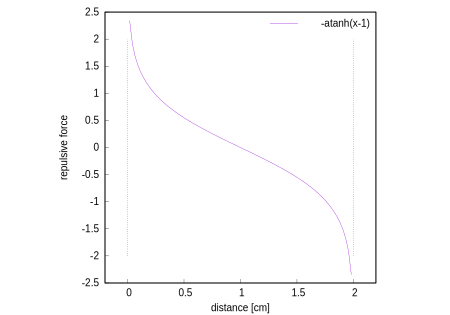
\includegraphics[width=1.0\hsize]{plot/minus_atanh.eps}
    \end{center}
    \caption{ほげほげ}
    \label{fig::atanh}
  \end{figure}

\subsection{画像認識}
  炎上ポールの認識には配布されたRapspberry Pi NoIR Camera V2(以下,カメラモジュール)を使用する.
  画像撮影から最も近い(と思われる)ポールへのベクトルを出力する一連の手順を,簡単に以下に示す.

  \begin{description}

    \item[画像取得] \mbox{} \\
      カメラモジュールへのアクセスには既成ライブラリ\cite{raspicam}を利用した.
      撮影によりピクセル値の2次元配列(cv::Mat)が出力として得られる.\\

    \item[カラーモデル変換] \mbox{} \\
      得られた画像のカラーモデルをRGBからHSVに変更する.\\

    \item[2値画像化] \mbox{} \\
      HSV画像データに対し赤色マスクをかけて2値画像に変換する.\\

    \item[ノイズ除去] \mbox{} \\
      モフォロジー処理によりノイズを除去する.\\

    \item[構造解析] \mbox{} \\
      2値画像中の輪郭線を検出した後,それを矩形で囲む.
      囲んだ矩形を縦横比で解析し,ポールの縦横比に対して$\pm 20 \%$以上の差があるものを除外する.

    \item[ベクトル作成]
      除外されず残った矩形の重心点を求め,
      カメラの画角を元に機体中心から重心点へ向かうベクトルを作る.\\

  \end{description}

\begin{thebibliography}{9}
  \bibitem{raspicam} "RaspiCam: C++ API for using Raspberry camera with/without OpenCV",\\
                     "\texttt{https://www.uco.es/investiga/grupos/ava/node/40}",2017年5月31日最終確認.
\end{thebibliography}

\end{document}
